\chapter{Versuch 4}
\label{chap:VERSUCH_4}

\section{Fragestellung, Messprinzip, Aufbau, Messmittel}
\label{chap:VERSUCH_4_FRAGESTELLUNG}

\subsection*{Fragestellung}
Aus den vorherigen Versuchen wurden verschiedene Berechnungen durchgeführt welche jetzt hier zusammen laufen. So geht es darum den aufgenommenen Grauwertkeil jetzt zu korrigieren mit den genannten Fehlern des Aufnahmesensors. 

\section{Auswertung}
\label{chap:VERSUCH_4_AUSWERTUNG}

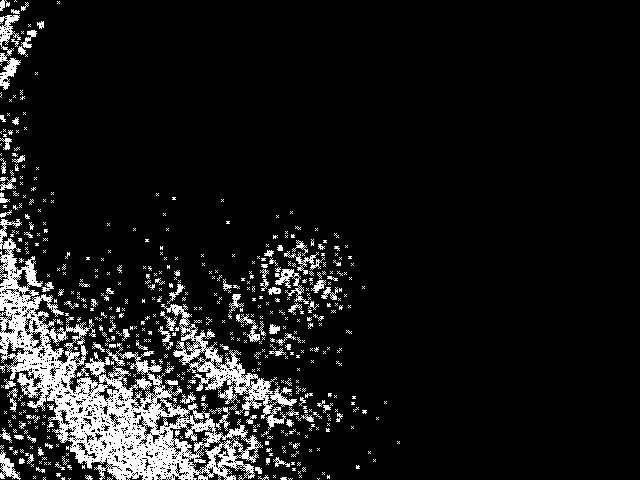
\includegraphics[scale=0.6]{media/dunkelContrastMax}

Wie man auf diesem Dunkelbild was Kontrast maximiert wurde gut erkennen kann, sind in der unteren linken Ecke nahezu alle Hot und Stuck Pixel(Alle Pixel die nicht den Wert 0 haben).

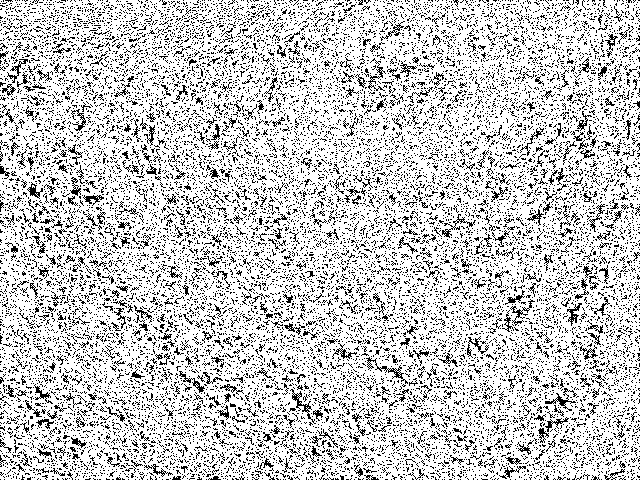
\includegraphics[scale=0.6]{media/weissContrastMax}

Hier ist das Gegenteil von dem Dunkelbild, ein Kontrast maximiertes Weißbild welches alle dead Pixels aufzeigt(Pixel die immer den wert 0 haben). Zusehen sind diese stärker in der unteren und oberen linken Ecke.

Aus diesen beiden Bildern wurde dann eine Kalibrierung durchgeführt mit dem ursprünglich erstelltem Bild von dem Grauwertkeil. Dabei wurde der Grauwertkeil minus dem Mittelwertbild des Dunkelbildes und anschließend minus dem normierten Mittelwertbild des Weißbildes gerechnet. Daraus folgen dann neue Werte des Grauwertkeils(Vorherige Werte siehe Tabelle Versuch 1):

\subsection*{Mittelwerte und Standardabweichung des Kalibrierten Grauwertkeilers}

\begin{tabular}{|c|c|c|}
\hline 
Graustufe & Mittelwert & Standardabweichung \\ 
\hline 
0 (schwarz) & 11.04 & 6.02 \\
\hline 
1 (dunkelgrau) & 81.14 & 8.1 \\ 
\hline 
2 (mittelgrau) & 150.12 & 8.85 \\ 
\hline 
3 (hellgrau) & 185.43 & 11.56 \\ 
\hline 
4 (weiß) & 214.03 & 14.37 \\ 
\hline 
\end{tabular} 
\captionof{table}{Tab:Grauwert2}
\newpage

\section{Interpretation}
\label{chap:VERSUCH_4_INTERPRETATION}
Wenn man den Grauwertkeil(vor und nach der Kalibrierung) jetzt miteinander vergleicht sieht man das sich fast überall die Standardabweichung verringert hat. Dies ist darauf zurück zu führen das wir aus den Grauwertkeil die Stuck, Hot und dead Pixels eliminiert haben durch die vorherige Versuche und Berechnungen.
Im allgemeinen folgt daraus ein einheitlicheres Bild ohne diese Störfaktoren und dies sieht dann folgender maßen aus:

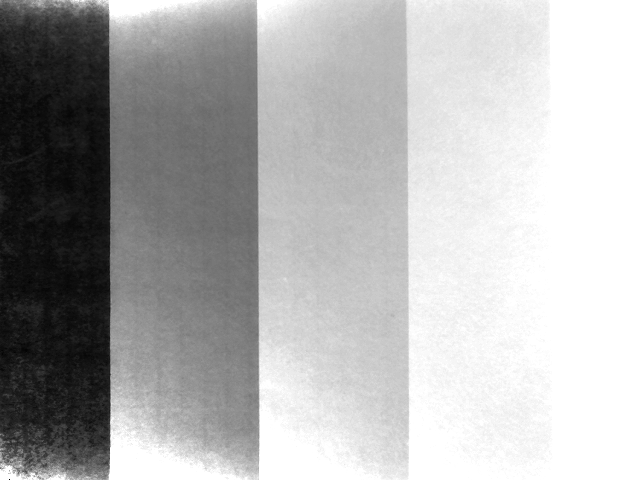
\includegraphics[scale=0.65]{media/grauWertKorrektur}